\documentclass[12pt]{article}

\usepackage{times}
\usepackage{textcomp}
\usepackage{listings}
\usepackage{fullpage}
\usepackage{color}
\usepackage{hyperref} 
\usepackage{pst-tree} 
\usepackage{verbatim} 
\usepackage{graphicx}
\usepackage{amsmath,amsfonts,amssymb,amsthm}
\graphicspath{ {./}}
\usepackage{courier}

\def\part#1{\item[\bf #1)]}
\renewcommand{\thesubsection}{Question \arabic{subsection}}
\lstset{language=C, keywordstyle={\bfseries \color{red}}, basicstyle=\footnotesize\ttfamily}

\author{Clement Tsang}

\begin{document}

\begin{center}
\Large\textbf{CS 241, Lecture 17 - Code Generation}
\end{center}

\section{Warm-up}
Consider the following WLP4 program, and write an equivalent MIPS program:
\begin{lstlisting}[mathescape, numbers=none, breaklines=true]
    int wain(int a, int b) {
        int c = a + b;
        return c * a;
    }
\end{lstlisting}
This code is valid and equivalent:   
\begin{lstlisting}[mathescape, numbers=none, breaklines=true]
    sw s1, -4(s30)
    sw s2, -8(s3)
    lis s4
    .word 4
    sub s30, s30, s4
    sub s30, s30, s4
    sub s30, s30, s4
    sw s0, 0(s30)
    lw s3, 8(s30)
    add s30, s30, s4
    add s30, s30, s4
    add s30, s30, s4
    jr s31
\end{lstlisting}

\section{Code Generation - Continued}
\begin{itemize}
    \item Recall our previous problem - that variables also have to go on the stack but we don't know what the offsets will be until we process ALL the variables and parameters if we use \$30 and offset from the top of the stack frame.
    \item Instead, we offset not from \$30, but \$29 - it now comes in use!  Remember that \$29 keeps track of the \textbf{bottom} of the stack frame! (note in normal MIPS, \$29 and \$30 are switched in functionality)
    \item We calculate offsets from \$29, which never changes, while \$30 does.
    \item So we can generate the following equivalent code:
\begin{lstlisting}[mathescape, numbers=none, breaklines=true]
int wain(int a, int b) { int c = 0; return a; }

lis s4
.word 4
sub s29, s30, s4
sw s1, -4(s30)
sub s30, s30, s4
sw s2, -4(s30)
sub s30, s30, s4
sw s0, -4(s30)   ; For int c = 0
sub s30, s30, s4
lw s3, 0(s29)    ; Offset in symbol table
add s30, s30, s4
add s30, s30, s4
add s30, s30, s4
jr s31
\end{lstlisting}
    \item This corresponds to the following \emph{new} offset table:\\
        \begin{center}
        \begin{tabular}{|c|c|c|}
            \hline
            Symbol & Type & Offset from \$29 \\
            \hline
            a & int & 0 \\
            b & int & -4 \\
            c & int & -8 \\
            \hline
        \end{tabular}\\
        \end{center}
    \item This is versus our \emph{old} offset table:\\
        \begin{center}
        \begin{tabular}{|c|c|c|}
            \hline
            Symbol & Type & Offset from \$30 \\
            \hline
            a & int & 8 \\
            b & int & 4 \\
            c & int & 0 \\
            \hline
        \end{tabular}\\
        \end{center}
    \item This also allows us to handle intermediate values of complicated arithmetic expressions by storing them on the stack, which would be impossible to feasibly do if relying on \$30.
    \item For example, what about a more complicated program?
\begin{lstlisting}[mathescape, numbers=none, breaklines=true]
int wain(int a, int b) {
    return a - b;
}
\end{lstlisting}
    \item Well, we already have the convention that \$3 stsores the output so we can use this for scratch work in between.  But this isn't enough - we need to load both a \emph{and} b.
    \item For convention, we also state \$5 stores intermediate work.
    \item Then, we could generate the following MIPS code:
\begin{lstlisting}[mathescape, numbers=none, breaklines=true]
lis s4
.word 4
sub s29, s30, s4
sw s1, -4(s30)
sub s30, s30, s4
sw s2, -4(s30)
sub s30, s30, s4
lw s3, 0(s29)    ; Offset in symbol table (a)
add s5, s3, s0   ; Store a in s5
lw s3, -4(s29)   ; Offset in symbol table (b)
sub s3, s5, s3
add s30, s30, s4 ; Restore stack 
add s30, s30, s4
jr s31
\end{lstlisting}
    \item However, things aren't all fine here - this approach breaks if we consider something like $a + (b - c)$.  We need to load $a$, then load $b$, then load $c$, compute $b - c$, then compute the final answer.  This needs \textbf{three} registers - and what will we do if we, say, add a fourth value $d$?  Four registers?  Five? 
    \item Instead, we will once again turn to our lord and saviour, the stack.  This way, we will only ever need two registers for scratch work!
    \item Our new code for the previous question:
\begin{lstlisting}[mathescape, numbers=none, breaklines=true]
int wain(int a, int b) { return a - b; }

lis s4
.word 4
sub s29, s30, s4
sw s1, -4(s30)
sub s30, s30, s4
sw s2, -4(s30)
sub s30, s30, s4
lw s3, 0(s29)       ; offset in symbol table (a)
sw s3, -4(s30)
sub s30, s30, s4    ; push a on stack
lw s3, -4(s29)      ; offset in symbol table (b)
add s30, s30, s4
lw s5, -4(s30)      ; pop from stack
sub s3, s5, s3
jr s31
\end{lstlisting}
    \item We use some shorthand for our code for simplicity.  We state:
\begin{lstlisting}[mathescape, numbers=none, breaklines=true]
code(a):
lw s3, N(s29)  ; N is the offset in the symbol table

push(s3):
sw s3, -4(s30)
sub s30, s30, s4

pop(s5):
add s30, s30, s4
lw s5, -4(s30)
\end{lstlisting}
    We are trying to find a function code(s) for every possible value in our grammar.
    \item For example:
\begin{lstlisting}[mathescape, numbers=none, breaklines=true]
int wain(int a, int b) {
    int c = 3;
    return a + (b - c);
}

lis s4
.word 4
sub s29, s30, s4
push(s1)
push(s2)
lis s5
.word 3
push(s5)
code(a)             ; Load a in s3
push(s3)            
code(b)             ; s3 <- b
push(s3)
code(c)             ; s3 <- c
pop(s5)             ; s5 <- b
sub s3, s5, s3      ; s3 <- b - c
pop(s5)             ; a <- s5
add s3,s5, s3       ; s3 <- a + (b - c)
jr s31
\end{lstlisting}
    \item We can generalize this technique so that we only need one extra register to store our components.
    \item We can generalize the above to our grammar.  Remember the rule $exprA exprB PLUS term$?  Then, we have:
\begin{lstlisting}[mathescape, numbers=none, breaklines=true]
exprA exprB PLUS term

code(exprA) = code(exprB) + push(s3) +
              code(term) + pop(s5) +
              add s3, s5, s3
\end{lstlisting}
    \item Note that above for the add command, term is in \$3 and expr is in \$5.
    \item Singleton grammars are easy to translate:
\begin{lstlisting}[mathescape, numbers=none, breaklines=true]
S -> BOF procedure EOF:
code(S) = code(procedure)

expr -> term:
code(expr) = code(term)
\end{lstlisting}
    \item Assignments are also not too bad for IDs (pointers are harder) (note N is the offset for exprA):
\begin{lstlisting}[mathescape, numbers=none, breaklines=true]
statement -> exprA BECOMES exprB SEMI: (if exprA is an ID):
code(statement) = code(exprB) + sw s3, N(s29) ; s3 <- exprB
\end{lstlisting}
\end{itemize}

\section{Importing Code and MERL}
\begin{itemize}
    \item A compiler needs to take lots of code from many different parts to work.
    \item We define a \emph{runtime environment (RTE)} as the execution environment provided to an application or software by the OS to assist programs in their execution, such as procedures, libraries, environment variables, etc.
    \item An example is msvcrt.dll, a module containing standard C library functions such as printf, memcpy, and so on, on Windows (for Linux this is libc.so).
    \item Therefore, it makes sense to provide print as part of the runtime.
    \item We are given MERL (MIPS Executable RElocatable Linkable) files.
    \item When we compile code, almost always what is output is not pure machine code - there is often some additional header information as well.  The object is usually \emph{object code}.
    \item These files can help us store additional information needed by the loader and linker.
    \item For example, we are provded with a print.merl file that we link with our assembled output:
\begin{lstlisting}[mathescape, numbers=none, breaklines=true]
./wlp4gen < source.wlp4 > source.asm
cs241.linkasm < source.asm > source.merl
linker source.merl print.merl > exec.mips
\end{lstlisting}
    \item Upon reaching the .mips file, we can call mips.twoints or mips.array!  We made it!
    \item To use print, we need to add .import print to the beginning of our file.  After this, we can print in our MIPS code!  It will print the contents of \$1, so you may need to save \$1 depending on waht you want.
    \item print also overwrites \$31!  We need to save and restore it!  The code thus looks like
\begin{lstlisting}[mathescape, numbers=none, breaklines=true]
code(println(expr);) = code(expr) + 
                       add s1, s3, s0 +
                       push (s31) +
                       lis s5 + .word print +
                       jalr s5 + pop(s31)
                       (+ lw s1, 0(s29)) ; depends on whether we stored this or not
\end{lstlisting}
    \item Which means that we've actually completed most of our statements, except for if, while, and delete!
    \item For the former two, we need to handle boolean tests...
    \item By convention, store ``1'' in \$11, so we have true and false stored somewhere.
    \item Also, store print in \$10.
    \item Our code structure therefore looks like this:
\begin{lstlisting}[mathescape, numbers=none, breaklines=true]
;Prologue
.import print
lis s4
.word 4
lis s10
.word print
lis s11
.word 1
sub s29, s30, s4
;end Prologue, begin Body
; space for variables
translated WLP4 code
;end Body and begin Epilogue
add s30, s29, 4
jr s31
\end{lstlisting}
\end{itemize}

\section{Boolean Tests, If, While}
\begin{itemize}
    \item How would we test a LT?
\begin{lstlisting}[mathescape, numbers=none, breaklines=true]
test -> exprA < exprB:
code(test) = code(exprA) +
             push(s3) + 
             code(exprB) +
             pop(s5) +
             slt s3, s5, s3
\end{lstlisting}
    \item Likewise, for GT:
\begin{lstlisting}[mathescape, numbers=none, breaklines=true]
test -> exprA < exprB:
code(test) = code(exprA) +
             push(s3) + 
             code(exprB) +
             pop(s5) +
             slt s3, s3, s5 ; Flip s3 and s5
\end{lstlisting}
    \item For NE:
\begin{lstlisting}[mathescape, numbers=none, breaklines=true]
test -> exprA < exprB:
code(test) = code(exprA) +
             push(s3) + 
             code(exprB) +
             pop(s5) +
             ;maybe store s6 and s7 if used
             slt s6, s3, s5 +
             slt s7, s5, s3 +
             ; Note 0 <= s6 + s7 <= 1
             add s3, s6, s7
\end{lstlisting}
    \item To do EQ, remember that $a == b$ is the same as $!(a != b)$, so we just need to negate our $!=$ result!:
\begin{lstlisting}[mathescape, numbers=none, breaklines=true]
test -> exprA < exprB:
code(test) = code(exprA) +
             push(s3) + 
             code(exprB) +
             pop(s5) +
             ;maybe store s6 and s7 if used
             slt s6, s3, s5 +
             slt s7, s5, s3 +
             ; Note 0 <= s6 + s7 <= 1
             add s3, s6, s7
             sub s3, s11, s3 ; Flip 0 to 1 and v.v.
\end{lstlisting}
    \item How about LEQ and GEQ?  Well, for LEQ, use the idea that $(a \leq b)$ is the same as $!(a > b)$.  The same holds for GEQ. 
    \item So we've covered all our tests!  Now to translate IF statements:
\begin{lstlisting}[mathescape, numbers=none, breaklines=true]
statement -> IF (test) {statements} ELSE {statements}:
code(statement) = code(test) +
                  beq s3, s0, else +
                  code(stmts1) +
                  beq s0, s0, endif +
                  else: code(stmts2) + 
                  endif :
\end{lstlisting}
    \item But there may be problems with multiple labels... how can we fix this?
    \item Easy!  Keep track of how many if statements we have with some counter.  Use label names like ``else\#'' and ``endif\#'' to keep track of which label we're on!  We did this with rustcc too.
    \item How about WHILE?
\begin{lstlisting}[mathescape, numbers=none, breaklines=true]
statement -> WHILE (test) {statements}:
code(statement) = loop: code(test) +
                  beq s3, s0, endWhile +
                  code(stmts) +
                  beq s0, s0, loop +
                  endWhile:
\end{lstlisting}
    \item Like IF, we need a while loop counter to track our while loops and label them accordingly!
    \item Note that we can generate COMMENTS with our MIPS code - DO THIS!  This will help a lot in deciphering wtf is going on with your generated code (remember this did WONDERS with rustcc).
\end{itemize}

\section{Recap}
\textbf{Conventions:}\\\\
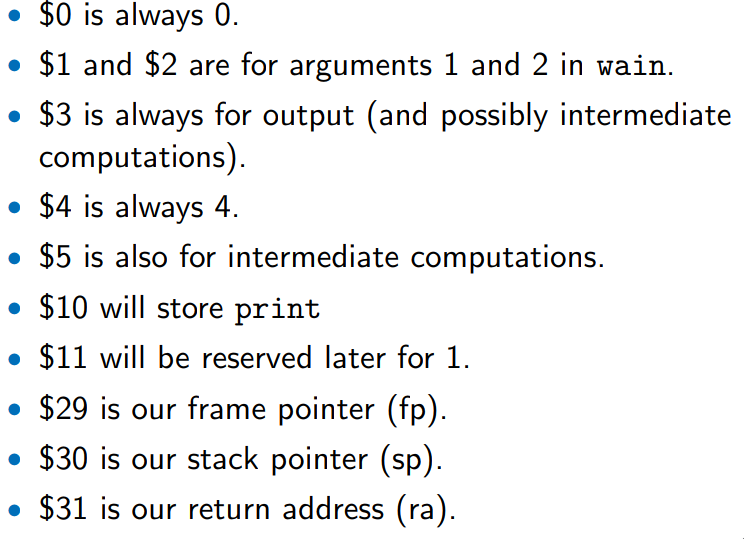
\includegraphics[scale=0.3]{conventions.png}\\
\textbf{Prologue:}\\\\
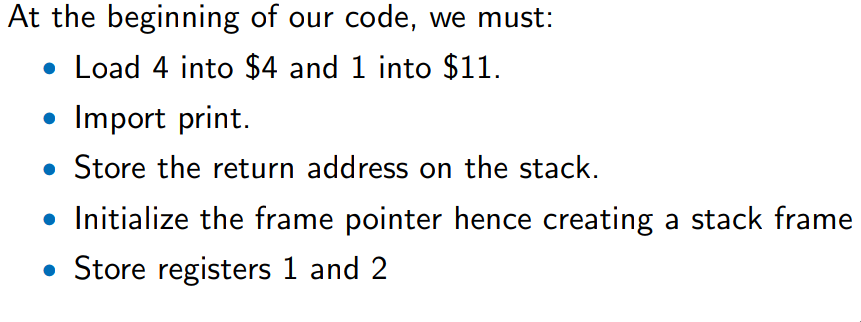
\includegraphics[scale=0.3]{prologue.png}\\
\textbf{Body:}\\\\
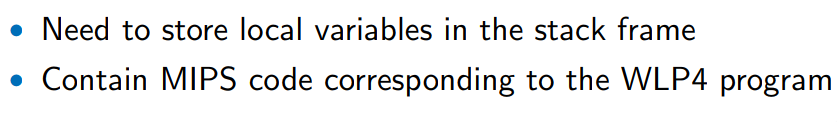
\includegraphics[scale=0.3]{body.png}\\
\textbf{Epilogue:}\\\\
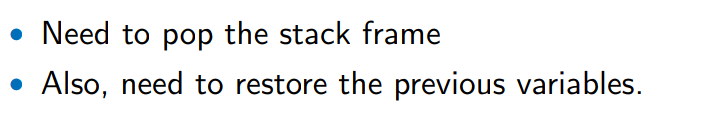
\includegraphics[scale=0.3]{epilogue.png}\\

\end{document}

